\chapter{Analisis}
\label{chap:analisis}

Pada bab ini akan dijelaskan mengenai analisis bentuk data, analisis bentuk visualisasi, analisis sistem visualisasi, dan perancangan modul.

\section{Analisis Bentuk Data}
Untuk dapat memvisualiasikan kurikulum 2018, diperlukan sumber data kurikulum 2018 yang terdapat pada github API. Untuk pengambilan datanya terdapat pada variable const fetchUsers dimana terdapat fungsi \textit{asynchronous} dengan kata kunci await untuk memanggil fungsi API web yang adalah fungsi \textit{fetch}.

\section{Analisis Bentuk Visualisasi}

\textit{Vis.js} memiliki 4 buah jenis visualisasi yaitu \textit{network}, \textit{timeline}, \textit{graph2d} dan \textit{graph3d}. Pada subbab ini akan dijelaskan jenis visualisasi apa yang dapat digunakan untuk memvisualisasikan kurikulum 2018.

\subsection{Graph2d}
\textit{Graph2d} menampilkan grafik dua dimensi, dimana terdapat dimensi horizontal (X) dan dimensi vertikal (Y). Sehingga gambar hanya dapat digeser ke kanan atau kiri dan atas atau bawah. Maka dari itu, \textit{grapgh2d} cocok untuk memvisualisasikan data yang bersifat \textit{continue} sedangkan, untuk data kurikulum 2018 kurang cocok karena bersifat diskrit.

\subsection{Graph3d}
\textit{Graph3d} menampilkan grafik tiga dimensi, dimana terdapat dimensi horizontal (X), dimensi vertikal (Y), dan dimensi kedalaman (Z). Sehingga gambar dapat melakukan rotasi dari berbagai perspektif. Maka dari itu, \textit{graph3d} kurang cocok untuk memvisualisasikan data kurikulum 2018 karena datanya tidak dapat direpresentasikan dalam bentuk ketiga dimensi tersebut.

\subsection{Timeline}
\textit{Timeline} menampilkan data dalam waktu, dimana data dapat berlangsung pada satu tanggal, atau memiliki tanggal mulai dan berakhir (rentang). Maka dari itu, \textit{timeline} cocok untuk membuat pohon kurikulum 2018, dimana kode matakuliah dapat dimodelkan dalam bentuk \textit{id}. Kemudian untuk nama matakuliah dapat dimodelkan dalam bentuk \textit{content} yang berbentuk kotak dengan warna :

\begin{itemize}
    \item biru muda untuk setiap matakuliah yang terdapat pada semester satu,
    \item kuning untuk setiap matakuliah yang terdapat pada semester dua,
    \item merah untuk setiap matakuliah yang terdapat pada semester tiga,
    \item hijau untuk setiap matakuliah yang terdapat pada semester empat,
    \item magenta untuk setiap matakuliah yang terdapat pada semester lima,
    \item ungu untuk setiap matakuliah yang terdapat pada semester enam,
    \item oranye untuk setiap matakuliah yang terdapat pada semester tujuh,
    \item biru tua untuk setiap matakuliah yang terdapat pada semester delapan.
\end{itemize}

Setiap \textit{content} akan dibagi kedalam dua grup menjadi matakuliah wajib yang terletak pada bagian atas \textit{timeline} dan matakuliah pilihan yang terletak pada bagian bawah \textit{timeline}. Visualisasi ini hanya akan memvisualisasikan lamanya masa kuliah yang seharusnya, yaitu selama empat tahun yang terdiri dari delapan semester. Untuk semester ganjil akan dimulai dari bulan Agustus sampai bulan Desember dan untuk semester genap akan dimulai dari bulan Januari sampai bulan Juli. Maka dari itu, besar \textit{content} akan mengikuti waktu untuk setiap semesternya.

\subsection{Network}
\textit{Network} menampilkan banyak jaringan yang terdiri dari banyak \textit{node} dan banyak \textit{edge}. Maka dari itu, \textit{network} cocok untuk membuat pohon kurikulum 2018, dimana kode matakuliah dapat dimodelkan dalam bentuk \textit{id}. Kemudian nama matakuliah dapat dimodelkan dengan label yang terdapat pada \textit{node} dengan warna :

\begin{itemize}
    \item biru muda untuk setiap matakuliah yang terdapat pada semester satu,
    \item kuning untuk setiap matakuliah yang terdapat pada semester dua,
    \item merah untuk setiap matakuliah yang terdapat pada semester tiga,
    \item hijau untuk setiap matakuliah yang terdapat pada semester empat,
    \item magenta untuk setiap matakuliah yang terdapat pada semester lima,
    \item ungu untuk setiap matakuliah yang terdapat pada semester enam,
    \item oranye untuk setiap matakuliah yang terdapat pada semester tujuh,
    \item biru tua untuk setiap matakuliah yang terdapat pada semester delapan.
\end{itemize}
\textit{Node} juga akan berbentuk kotak untuk mata kuliah wajib dan berbentuk lingkaran untuk mata kuliah pilihan. Untuk matakuliah a yang memiliki prasyarat b dapat dimodelkan dengan \textit{edges} berarah dari \textit{node} b ke \textit{node} a. Terdapat tiga macam edges yang warnanya mengikuti warna \textit{node}nya, yaitu :
\begin{enumerate}
    \item edges yang berbentuk garis dengan ujung anak panah yang melambangkan prasyarat tempuh.
    \item edges yang berbentuk garis putus - putus dengan ujung anak panah yang melambangkan prasyarat lulus.
    \item edges yang berbentuk garis putus - putus saja yang melambangkan prasyarat bersamaan.
\end{enumerate}
Terdapat delapan buah node tambahan yang berisikan semester satu sampai semester delapan secara naik berurutan ke bawah yang berfungsi untuk mengelompokkan \textit{node} - \textit{node} untuk setiap semesternya.

\section{Analisis Sistem Visualisasi}

\subsection{Spesifikasi Kebutuhan Perangkat Lunak}
Sesuai dengan rumusan masalah, perangkat lunak yang dibangun hanya akan mengolah data menjadi bentuk visualisasi yang paling cocok untuk memvisualisasikan kurikulum 2018. Perangkat lunak yang dibangun akan menggunakan \textit{framework} \textit{Electron} dan pustaka \textit{Vis.js}. Pertama - tama perangkat lunak akan mengambil data kurikulum 2018 dari \textit{API}. Kemudian data yang diambil akan diolah kedalam bentuk visualisasi \textit{Network} dan \textit{Timeline}, dimana kedua bentuk visualisasi tersebut merupakan bentuk yang paling cocok untuk memvisualisasikan kurikulum 2018.

Perangkat lunak ini dapat berjalan di berbagai sistem operasi. Sesuai dengan kemampuan framework \textit{Electron} yang merupakan aplikasi lintas platform, maka pada penelitian ini akan menggunakan sistem operasi \textit{Windows}. Namun, perangkat lunak akan tetap dapat berjalan pada sistem operasi \textit{Linux} maupun \textit{MacOs}.

\subsection{Use Case Diagram}
\begin{figure}[H]
    \centering
    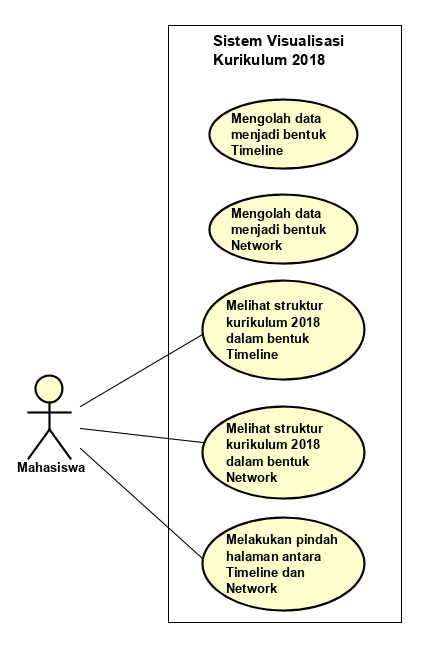
\includegraphics[width=6cm, height=10cm]{Gambar/Use Case.jpg}
    \caption{Use Case Diagram}
    \label{fig:gambarUseCase}
\end{figure}

Pada diagram \textit{use case} (gambar : \ref{fig:gambarUseCase}) terdapat tiga fitur bagi mahasiswa yaitu, melihat struktur kurikulum 2018 dalam bentuk \textit{Timeline}, melihat struktur kurikulum 2018 dalam bentuk \textit{Network}, dan melakukan pindah halaman antara \textit{Timeline} dan \textit{Network}. Selanjutnya bagi sistem, terdapat 2 fitur yaitu, mengolah data dalam bentuk \textit{Timeline} dan mengolah data menjadi bentuk \textit{Network}. 

\textbf{\textit{Scenario Use Case}}

\begin{itemize}
    \item Sistem akan mengambil data dari \url{https://raw.githubusercontent.com/ftisunpar/data/master/prasyarat.json}.
    \item Sistem mengolah data menjadi bentuk \textit{Timeline}.
    \item Sistem mengolah data menjadi bentuk \textit{Network}.
    \item Mahasiswa melihat struktur kurikulum 2018 dalam bentuk \textit{Timeline}.
    \item Mahasiswa melihat struktur kurikulum 2018 dalam bentuk \textit{Network}.
    \item Mahasiswa dapat melakukan pindah halaman antara halaman \textit{Timeline} dengan halaman \textit{Network}.
\end{itemize}

\subsection{Perancangan Modul}
\begin{itemize}
    \item Pada berkas \textit{JavaScript} \textit{network} terdiri dari:
    \begin{itemize}
        \item \textbf{fungsi \textit{processNetwork}}, dimana merupakan fungsi utama yang akan menjalankan fungsi - fungsi lainnya, seperti :
        \begin{itemize}
            \item \textbf{fungsi \textit{fetchUsers}}, yang akan menjalankan fungsi \textit{async} dengan kata kunci await ditambah dengan fungsi \textit{fetch} yang berfungsi untuk meminta dan mengambil data dari API.
            Untuk kodenya dapat dilihat pada Kode \ref{lst:kodeAmbilData}.
            
            \newpage
            \begin{lstlisting}[language=JavaScript, caption=Kode pengambilan data dari API\label{lst:kodeAmbilData}]
            let matkul = '';
            const fetchUsers = async () => {
                try {
                    const res = await fetch('https://raw.githubusercontent.com/ftisunpar/data/master/prasyarat.json');
                    if (!res.ok) {
                        throw new Error(res.status);
                    }
                    const data = await res.json();
                    matkul = data;
                    createNetwork();
                } catch (error) {
                    console.log(error);
                }
            }
            \end{lstlisting}
            
            \item \textbf{fungsi \textit{createNetwork}}, yang berfungsi untuk mengolah data yang telah diambil dari API menjadi sebuah visualisasi yang berbentuk \textit{network}. Di dalam fungsi ini terdapat sebuah \textit{looping} untuk membuat delapan buah \textit{node} yang berisikan semester satu sampai dengan semester delapan yang berfungsi sebagai patokan untuk penempatan setiap node mata kuliah sesuai dengan letak semesternya. Selanjutnya terdapat sebuah \textit{looping} untuk membuat \textit{node} - \textit{node} sesuai dengan jumlah mata kuliah, dimana untuk bentuk dan posisi \textit{node}nya akan diatur di dalamnya. Pada \textit{looping} ini juga akan dibuatkan \textit{edges} untuk setiap \textit{node}nya sesuai dengan prasyaratnya masing - masing, dimana untuk bentuk \textit{edges}nya akan diatur di dalamnya. Tidak ada fungsi khusus yang dibuat untuk memberi warna pada setiap \textit{node} yang ada, karena warna \textit{node} akan diberikan secara otomatis oleh \textit{library} \textit{Vis.js}. Untuk kodenya dapat dilihat pada Kode \ref{lst:kodeMembuatNetwork}.
            
            \begin{lstlisting}[language=JavaScript, caption=Kode untuk membuat Visualisasi Network\label{lst:kodeMembuatNetwork}]
            const horizontal = [];
            for (i = 1; i < 9; i++) {
                nodes.add([{
                    id: i, label: "Semester " + i, group: i, y: i*150
                }])
                if (i != 8) {
                    edges.add([
                        { from: i, to: i + 1 }
                    ])
                }
                horizontal[i] = 0;
            }
            
            for (let i = 0; i < matkul.length; i++) {
                let shape=""
                if(matkul[i].wajib){
                    shape="box"
                }
                else{
                    shape="circle"
                }
    
                horizontal[matkul[i].semester] += 200; 
                nodes.add([{
                    id: matkul[i].kode, label: matkul[i].nama, group: matkul[i].semester, 
                    x:horizontal[matkul[i].semester], y: matkul[i].semester*150, shape:shape 
                }])
    
                if(matkul[i].prasyarat.tempuh.length != 0){
                    for (let j = 0; j < matkul[i].prasyarat.tempuh.length; j++){
                        edges.add([
                            { from: matkul[i].kode, to: matkul[i].prasyarat.tempuh[j], 
                              arrows: "from"}
                        ])
                    }
                }
                if(matkul[i].prasyarat.lulus.length != 0){
                    for (let j = 0; j < matkul[i].prasyarat.lulus.length; j++){
                        edges.add([
                            { from: matkul[i].kode, to: matkul[i].prasyarat.lulus[j], 
                              dashes: true }
                        ])
                    }
                }
                if(matkul[i].prasyarat.bersamaan.length != 0){
                    for (let j = 0; j < matkul[i].prasyarat.bersamaan.length; j++){
                        edges.add([
                            { from: matkul[i].kode, to: matkul[i].prasyarat.bersamaan[j], 
                              arrows: "from", dashes: true }
                        ])
                    }
                }
            }
            \end{lstlisting}
            
        \end{itemize}
    \end{itemize}

    \item Pada berkas \textit{javascript} \textit{timeline} terdiri dari: 
    \begin{itemize}
        \item \textbf{fungsi \textit{processTimeline}}, dimana merupakan fungsi utama yang akan menjalankan fungsi - fungsi lainnya, seperti :
        \begin{itemize}
            \item \textbf{fungsi \textit{fetchUsers}}, yang akan menjalankan fungsi \textit{async} dengan kata kunci await ditambah dengan fungsi \textit{fetch} yang berfungsi untuk meminta dan mengambil data dari API.
            Untuk kodenya dapat dilihat pada Kode \ref{lst:kodeAmbilData}.
            
            \item \textbf{fungsi \textit{createTimeline}} yang berfungsi untuk mengolah data yang telah diambil dari API menjadi sebuah visualisasi yang berbentuk \textit{timeline}. Di dalam fungsi ini terdapat sebuah \textit{variable groups} yang berfungsi untuk membuat dua \textit{group} yaitu mata kuliah wajib dan mata kuliah pilihan yang akan muncul pada bagian sisi kiri (sumbu y) \textit{timeline}. Selanjutnya terdapat fungsi \textit{Date} untuk mengambil data tahun dan bulan saat ini, dimana akan digunakan untuk menentukan waktu yang akan muncul pada bagian sisi bawah (sumbu x) \textit{timeline}. Selanjutnya terdapat sebuah \textit{looping} untuk mengisi \textit{array} semester di mana setiap arraynya akan berisi informasi tentang bulan dan tahun untuk setiap semesternya. Kemudian terdapat sebuah \textit{looping} untuk membuat \textit{content} sesuai dengan jumlah mata kuliah, dimana warna, ukuran, dan letak \textit{content} akan diatur di dalamnya. Untuk kodenya dapat dilihat pada Kode \ref{lst:kodeMembuatTimeline}.
            
            \begin{lstlisting}[language=JavaScript, caption=Kode untuk membuat Visualisasi Network\label{lst:kodeMembuatTimeline}]
              var groups = new vis.DataSet([
                { id: 1, content: "Mata Kuliah Wajib" },
                { id: 2, content: "Mata Kuliah Pilihan" },
              ]);
        
              let tahun=new Date().getFullYear();
              let bulan = new Date().getMonth();
              if(bulan<7){
                tahun-=1
                bulan=7
              }
              else{
                bulan=7
              }
        
              let semester=[]
              for(i=1;i<=9;i++){
                  semester[i]= tahun.toString()+"-"+bulan.toString()+"- 31"
                  if(i%2!=0){
                    bulan+=5
                  }
                  else{
                    bulan-=5
                    tahun+=1
                  }
              }
        
              var res = [];
              let color=["","lightBlue","yellow","red","green","pink","purple","orange","darkBlue"]
              for (var i = 0; i < matkul.length; i++) {
                  let wajib=''
                  if(matkul[i].wajib){
                    wajib=1;
                  }
                  else{
                    wajib=2;
                  }
                  res.push(
                    { id: matkul[i].kode, content: matkul[i].nama, editable: false,group:wajib , 
                      start: semester[matkul[i].semester],end:semester[matkul[i].semester+1], 
                      className: color[matkul[i].semester]  }
                  )
              }
              var items = new vis.DataSet(res);
              
              var container = document.getElementById('timeline');
        
              var options = {};
        
              var timeline = new vis.Timeline(container, items,groups, options); 
            }
            fetchUsers();
            \end{lstlisting}
            
        \end{itemize}
    \end{itemize}
\end{itemize}
 

